\section{Results}
\label{sec:results}

We provide several types of results.
First, we show that the novel expected-loss (EL) estimator performs best in our validation assays.
Second, qualitative exploratory analysis confirms that the Cre-specific connectivity matrices generated using this model are consistent with known biology. 
Third, statistical decomposition of the wild-type connectivity matrix using unsupervised learning shows how archetypal components can combine to produce observed signals.

\subsection{Model evaluation}
\label{sec:model_eval}

Our EL model generally performs better than the other estimators that we consider.
Table \ref{tab:crossvalidation} contains weighted losses from leave-one-out cross-validation of candidate models, such as the NW Major-WT model from  \citet{Knox2019-ot}.
The EL model combines the good performance of class-specific models like NW Leaf-Cre in regions like Isocortex with the good performance of class-agnostic models in regions like Thalamus.
Additional information on model evaluation, including class and structure specific performance, is given in Appendix \ref{supp_sec:model-evaluation}.
In particular, Supplementary Table \ref{tab:eval_size} contains the sizes of these evaluation sets in each major structure, and Supplementary Section \ref{supp_sec:loss_subsets} contains the structure- and class specific losses.

\begin{table}[H]
\small
\begin{tabular}{lrrrrrrr}
\toprule
& Mean Leaf-Cre & NW Major-Cre& NW Leaf-Cre & NW Leaf &NW Major-WT  & NW Major & EL \\
$\widehat f$ &           Mean & \multicolumn{5}{l}{NW} &     EL \\
$\mathcal D$ & $I_c \cap I_L$ & $I_c \cap I_M$ & $I_c \cap I_L$ &  $I_L$ & $I_{wt} \cap I_M$ &  $I_M$ &  $I_L$ \\
\midrule
Isocortex &          0.239 &          0.252 &          0.234 &  0.279 &             0.274 &  0.274 & \textbf {0.228} \\
OLF       &          0.193 &          0.233 &          0.191 &  \textbf{0.135} &             0.179 &  0.179 &  0.138 \\
HPF       &          0.175 &          0.332 &          0.170 &  0.205 &             0.228 &  0.228 & \textbf {0.153} \\
CTXsp     &       \textbf   {0.621} &          \textbf{0.621} &         \textbf {0.621} & \textbf {0.621} &            \textbf {0.621} &  \textbf {0.621} &  \textbf{0.621} \\
STR       &          0.131 &         \textbf {0.121} &          0.128 &  0.169 &             0.232 &  0.232 &  0.124 \\
PAL       &          0.203 &          0.205 &          0.203 &  0.295 &             0.291 &  0.291 &  \textbf{0.188} \\
TH        &          0.673 &          0.664 &          0.673 & \textbf {0.358} &             0.379 &  0.379 &  0.369 \\
HY        &          0.360 &          0.382 &          0.353 &  0.337 &             0.317 &  0.317 &  \textbf{0.311} \\
MB        &          0.168 &          0.191 &          0.160 &  0.199 &             0.202 &  0.202 & \textbf {0.159} \\
P         &          0.292 &          0.292 &          0.292 &  0.299 &             0.299 &  0.299 &  \textbf{0.287} \\
MY        &          0.268 &          0.347 &          0.268 &  0.190 &            \textbf{ 0.189 }& \textbf {0.189} &  0.204 \\
CB        &      \textbf {   0.062} &        \textbf { 0.062 }&         \textbf {0.062 }&  0.068 &             0.112 &  0.112 &  0.068 \\
\bottomrule
\end{tabular}
\caption{Losses from leave-one-out cross-validation of candidate models. \textbf{Bold} numbers are best for their major structure.}
\label{tab:crossvalidation}
\end{table}



%results sligghtyl differnet - why ?
\newpage

\subsection{Connectivities}

Our main result is the estimation of matrices $\hat {\mathcal C}_v \in \mathbb R_{\geq 0}^{S \times T}$ representing connections of source structures to target structures for particular cre-lines $v$. 
We confirm the detection of several well-established connectivities within our tensor, although it is our expectation that additional interesting biological processes are also manifest.
The connectivity tensor and code to reproduce it are available at \url{https://github.com/AllenInstitute/mouse_connectivity_models/tree/2020}.
%Note that many entries of these matrices are missing due to lack of experiments.

\subsubsection{Overall connectivity}

Several expected biological processes are evident in the wild-type connectivity matrix $\mathcal C_{wt}$ from leaf sources to leaf targets shown in Figure \ref{fig:full_wt}.
Intraareal connectivities are clear, as are ipsilateral connections between cortex and thalymus.
The clear intrastructural and intraareal connectivities mirror previous estimates in \citet{Oh2014-kh} and \citet{Knox2019-ot} and descriptive depictions of individual experiments in \citet{Harris2019-mr}.
These short-range connectivities define a 

Our estimated wild-type connectivities appear more variable than those in \citet{Knox2019-ot}, which used the NW Major-WT model whose accuracy is evaluated in Table \ref{tab:crossvalidation}.
This is plausibly because of both the layer-specific targeting of the different cre-lines, and also the layer-specificity of the selected model.
Although layer-specificity is a major advantage of including distinct cre-lines, for comparison, we also plot coarser projections between summary-structure sources and targets in the cortex in Figure \ref{fig:cortex_wt}.
These are averages over component layers weighted by layer size.
Grossly congruent with the previous work, these results also exhibit a larger range of connectivities than those in \citet{Knox2019-ot}.
Importantly, as shown in Table \ref{tab:crossvalidation} this finer spatial resolution corresponds to the increased accuracy of our EL model over the NW Major-WT model.

\newpage

\begin{figure}[H]
\centering
    \subfloat[] {
    \label{fig:full_wt}
    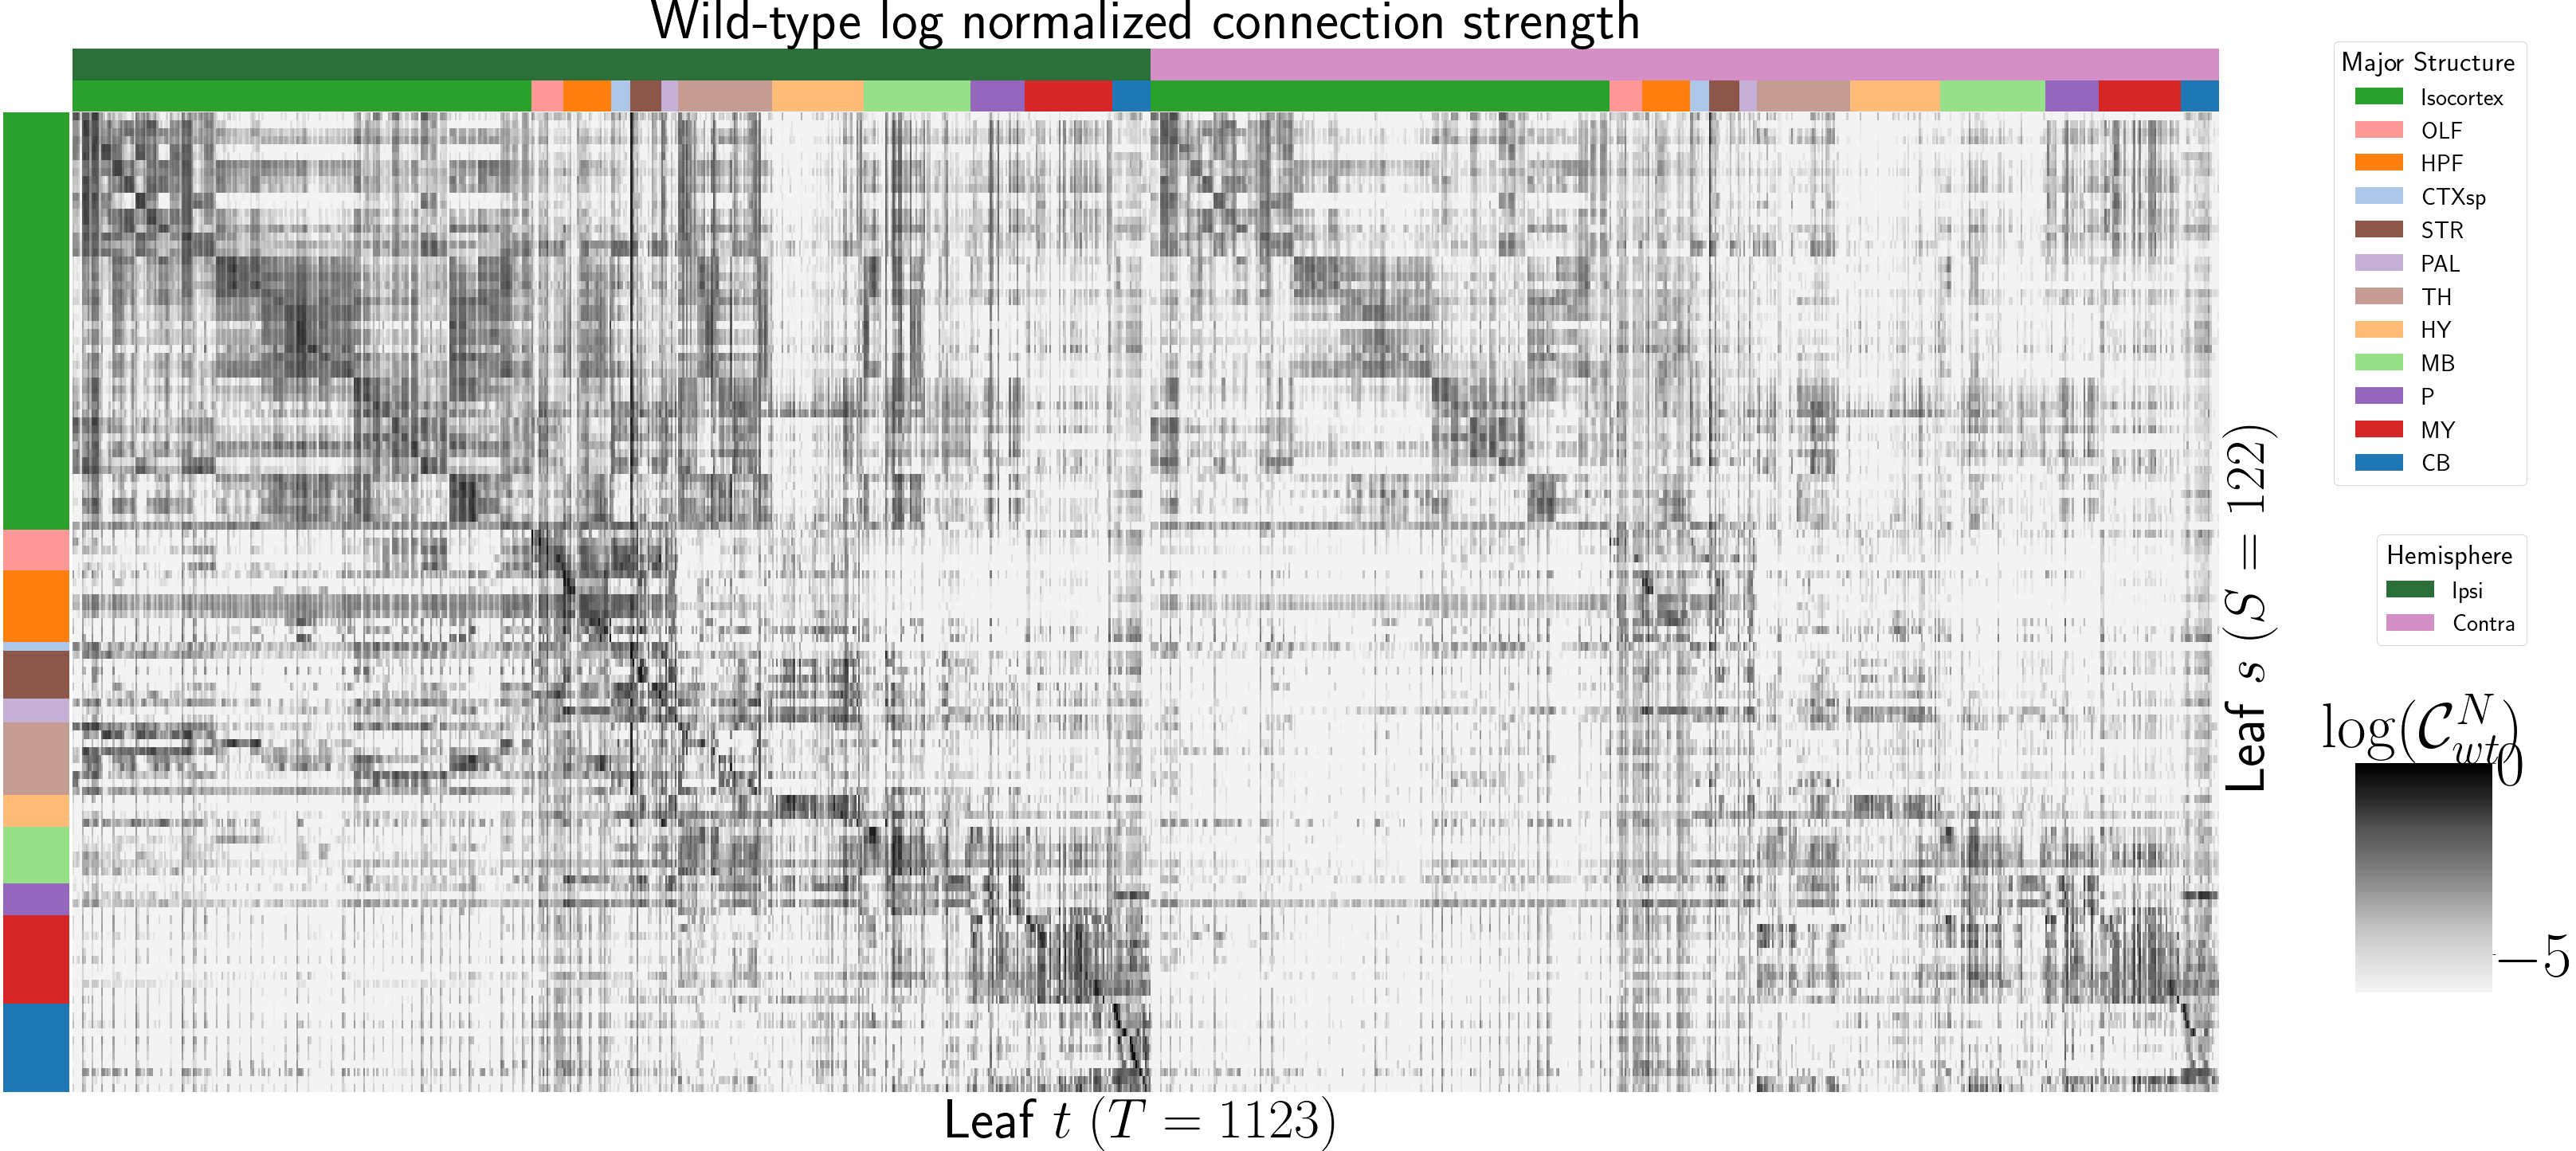
\includegraphics[width = \textwidth]{figs/conn_leaf2.png}
    } 
        \newline
       \subfloat[] {
    \label{fig:cortex_wt}
    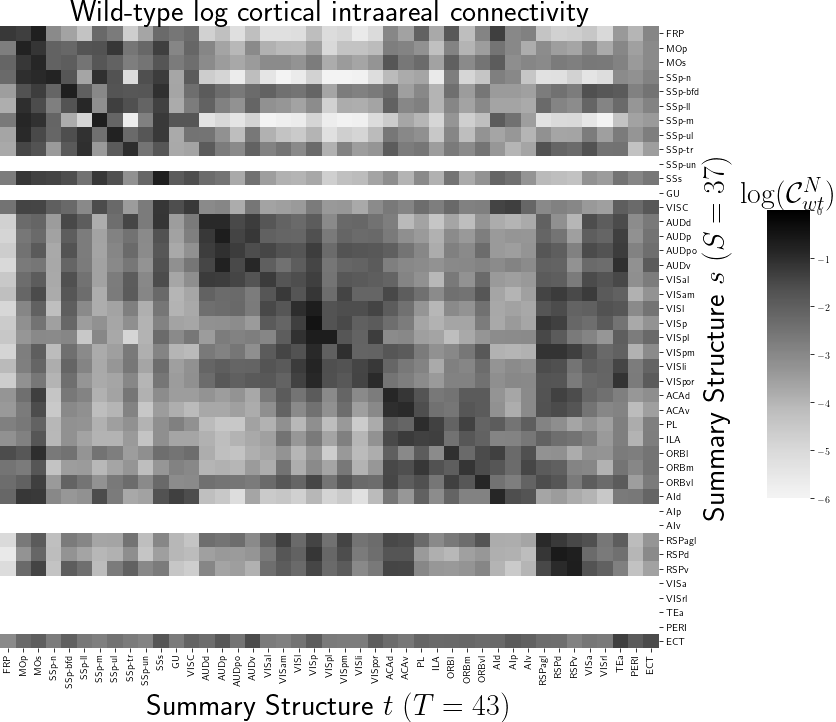
\includegraphics[width = .5\textwidth]{figs/conn_sum_cortex.png}
    } 
   \caption{Wild-type connectivities.
   \ref{fig:full_wt} Log wild-type connectivity matrix $\log \mathcal {C} (s,t,v_{wt})$.
   \ref{fig:cortex_wt} Log wild-type intracortical connectivity matrix at the summary structure level.}
   \label{fig:connectome}
\end{figure}

\newpage
\subsubsection{Class-specific connectivities}

Source and cell-type combinations which project similarly indicate the network structure underpinning cognition.
Our estimates of these class-specific connectivities exhibit certain known behaviors.
In Figure \ref{fig:data_ct}, we display results for the VISp and MO cortical areas.
These are ideal testbeds for our connectivities because they have well-established layer-specific projection patterns that can be detected with our layer-specific cre-line based targeting \citet{Jeong2016-dc}, and are also well-represented in our dataset.

Our results are consistent with anterograde tracing experiments outside our dataset \citet{Jeong2016-dc}.
Figure \ref{fig:ct_spc} shows that in VISp, the Ntsr1-Cre line strongly targets the thalymic LP nuclei, and in MO, layer 5 projects to anterior basolateral amygdala (BLA) and capsular central amygdala (CEA), while layer 6 does not.
Recall that we display connectivity estimates for structures with at least one injection centroid in the structure.
Thus, the position of non-zero rows in Figure \ref{fig:ct_spc} shows the localization of Rbp4-Cre and Ntsr1-Cre injection centroids to layers 5 and 6 respectively (this is further examined in Supplemental Section \ref{sec:data}).
Thus, as a heuristic alternative model, to also synthesize information about leafs targeted by different cre-lines, we also generate an average connectivity matrix over all cre-lines.
This model is not evaluated in our testing, and is only a general stand-in for overall behavior, but provides a useful summary of results.

Cell-class, while often correlated with cortical layer, is often a stronger driver of connectivity than summary structure.
Figure \ref{fig:ct_clust} shows a collection of connectivity strengths generated using cre-specific models for wild-type, Cux2, Ntsr1, Rbp4, and Tlx3 cre-lines from visual signal processing leafs in the cortex to cortical and thalymic nucleii.
We use heirarchical clustering to sort source structure/cell-class combinations by the similarity of their structural projections, and sort target structures by the structures from which they receive projections.
Examining the former, we can see that the Ntsr1 Cre-line distinctly projects to thalymic nucleii, regardless of summary structure.
This contrasts with the tendency of other cell-classes to project intracortically in a manner determined by the source structure.
Similarly, layer 6 targets are not strongly projected to by any of the displayed Cre-lines.
There are too many targeted summary structures to plot here, but we expect that the source profile of each target clusters by structure.

\newpage

\begin{figure}[H]
\subfloat[]{
\label{fig:ct_spc}
    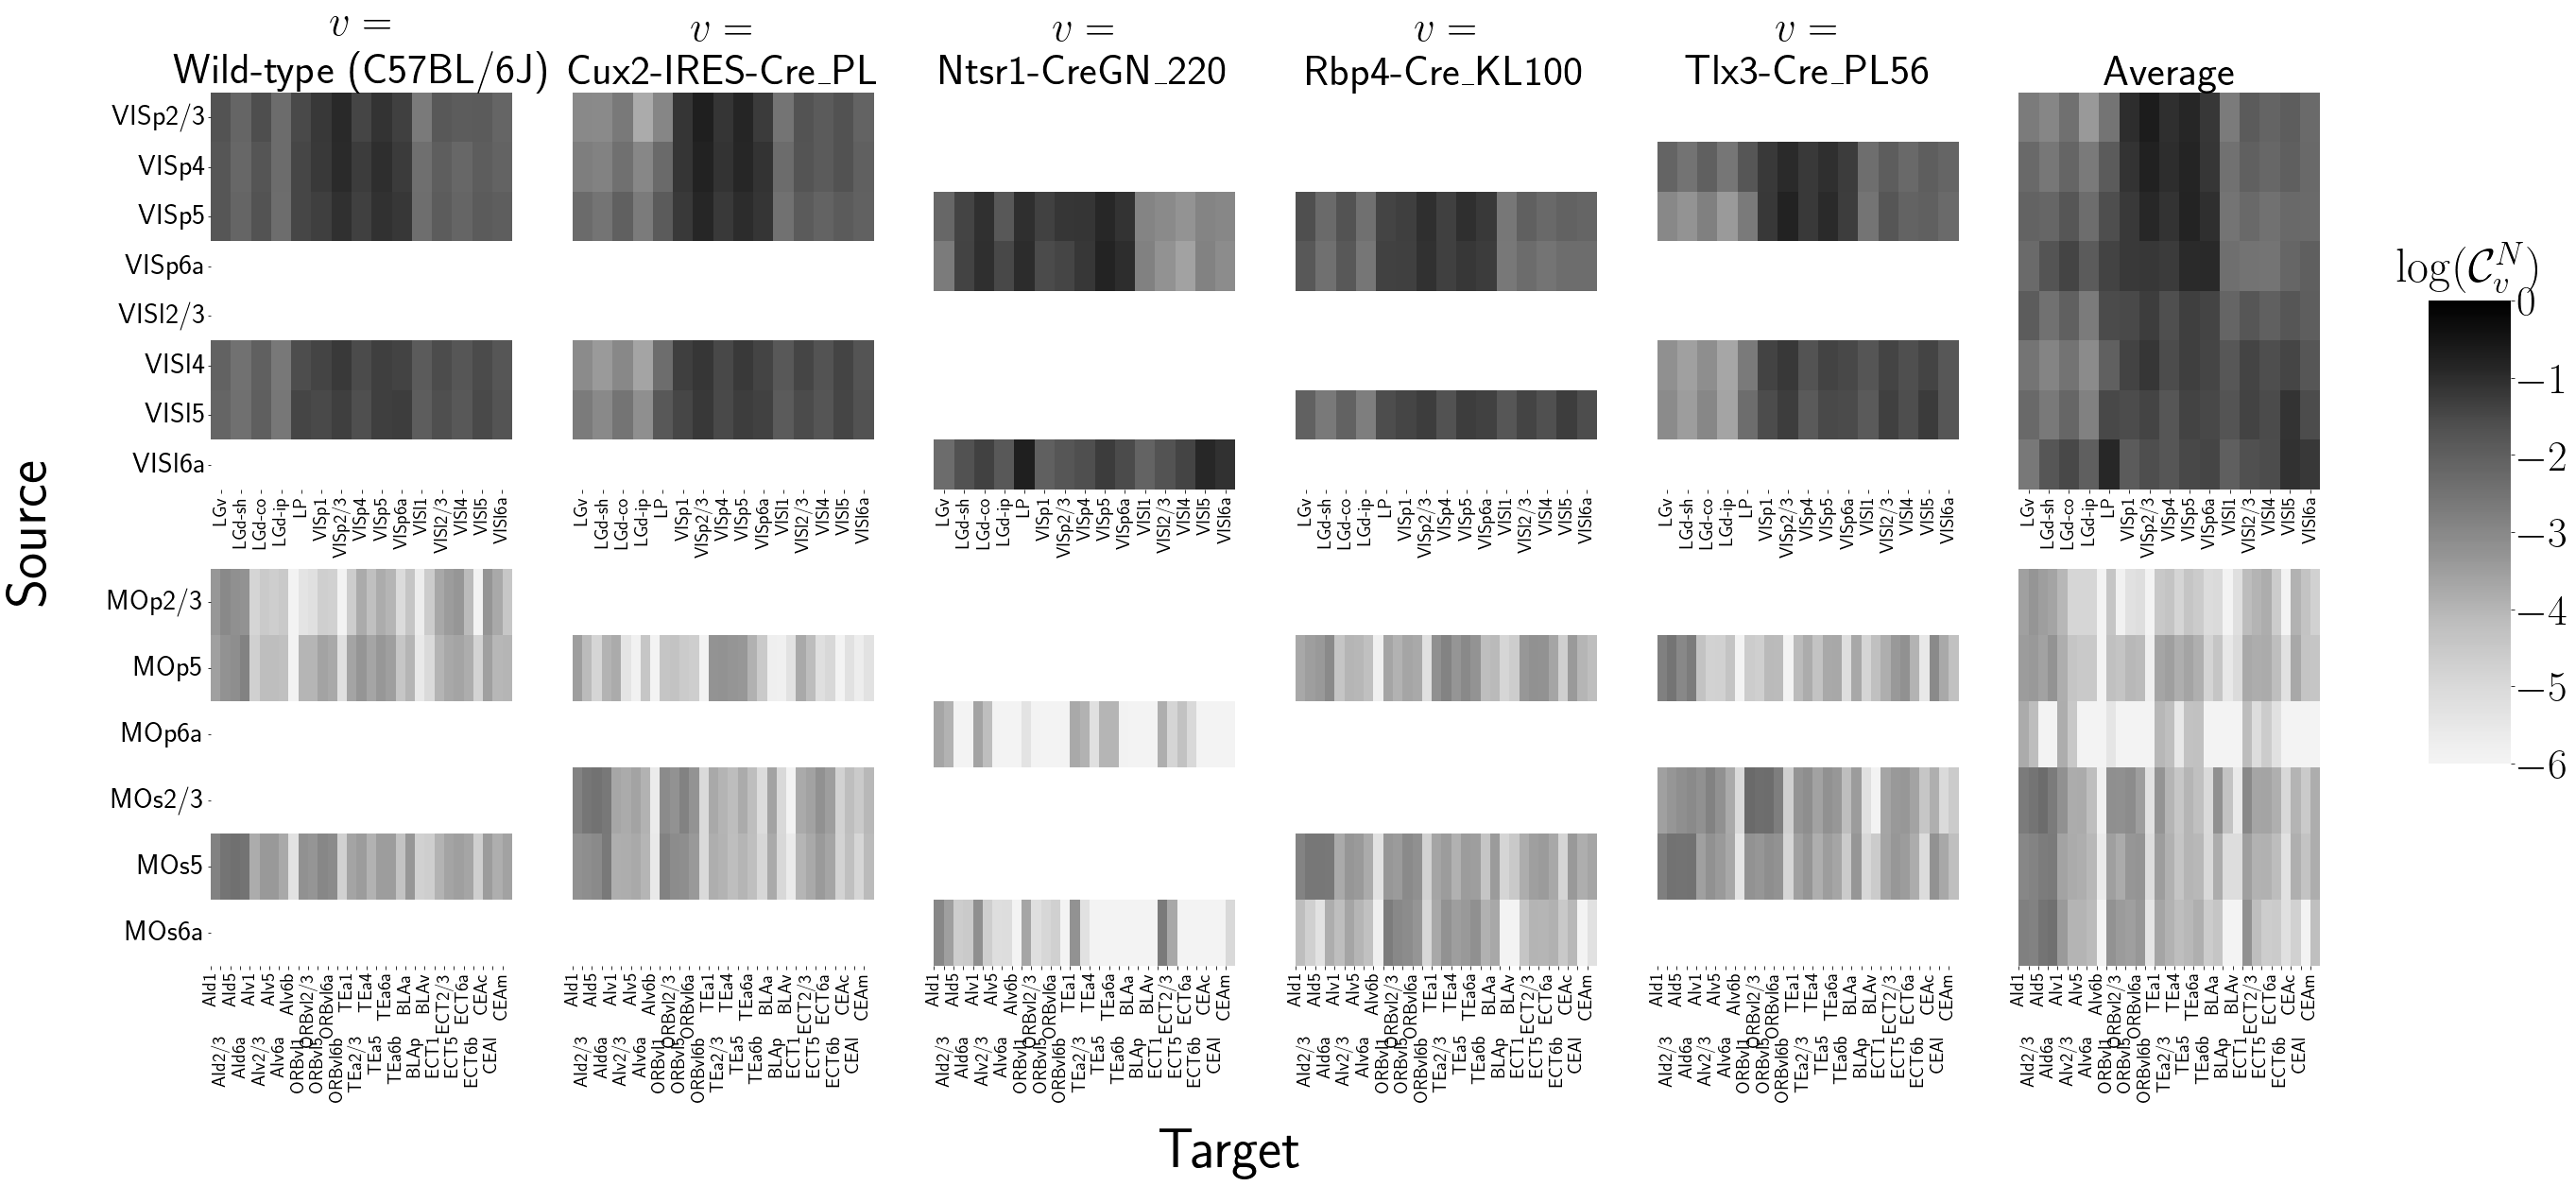
\includegraphics[width=.8\textwidth]{figs/visp_mo.png} 
    }
    \newline
 \subfloat[]{
 \label{fig:ct_clust}
    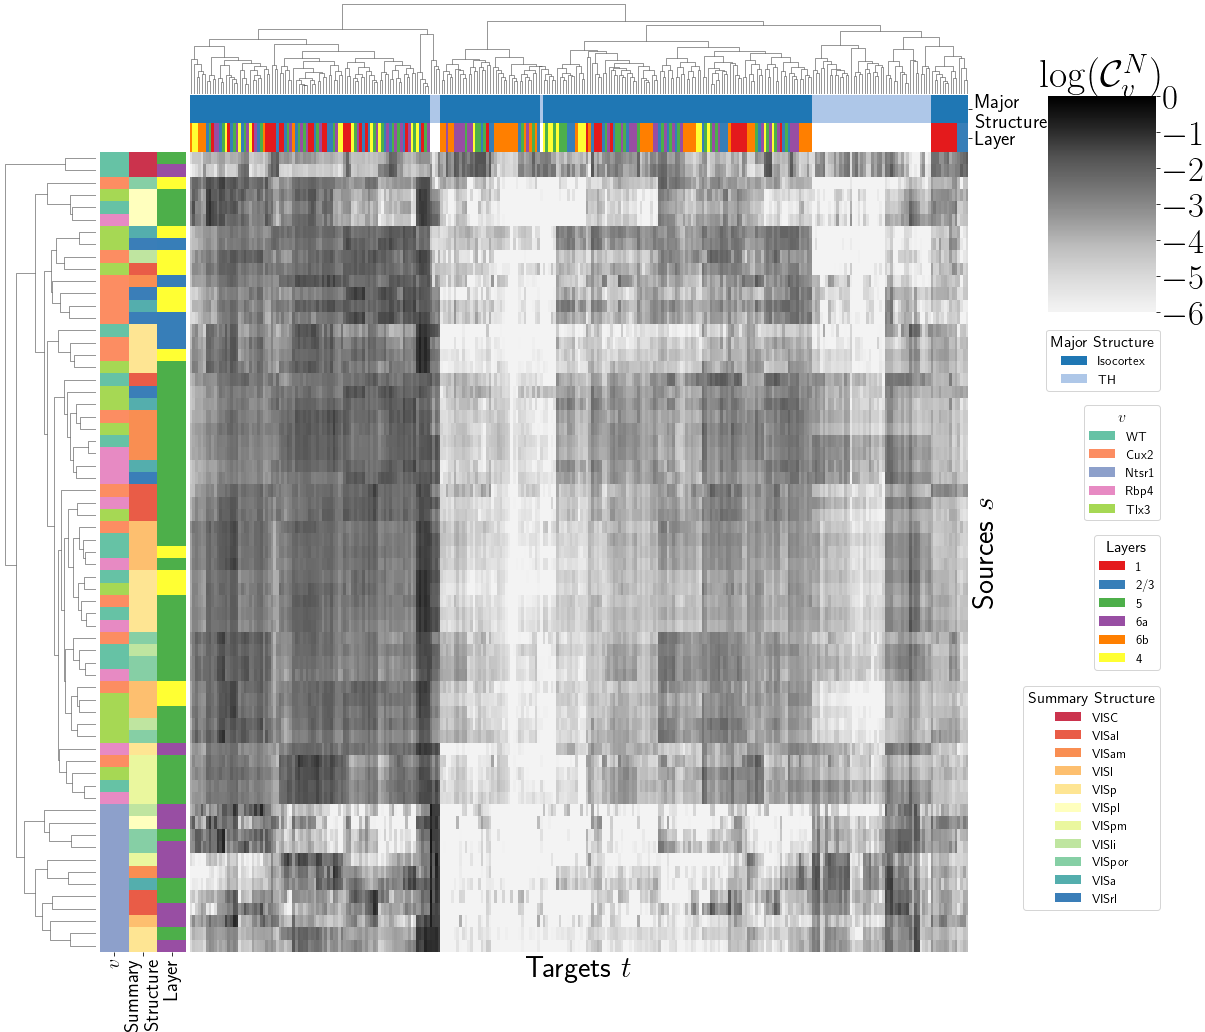
\includegraphics[width=.6\textwidth]{figs/heirarchical.png}
    }
    
    \caption{  Cell-class specificity. \ref{fig:ct_spc} Selected cell-class and layer specific connectivities from VISp and MO.
	 Sources without a injection of that Cre-type are not estimated due to lack of data for that Cre-line in that structure.
    		\ref{fig:ct_clust}
		Heirarchical clustering of connectivity strengths from visual signal processing cell-types to cortical and thalymic targets.
		Cre-line, summary structure, and layer are labelled on the sources.
		Major brain division and layer are labelled on the targets.}
\label{fig:data_ct}
\end{figure}

\newpage

\subsection{Connectivity Analyses}

Each structural connectivity matrix is a high-dimensional realization of relatively few biological processes, and decomposition of neural signals to recover these processes is a fundamental goal in neuroscience.
In this section, we apply non-negative matrix factorization to decompose the long-range wild-type connectivities into linear combinations of archetypal connectivities.
This decomposes the remaining censored connectivity matrix into a linear model based off a relatively small number of distinct signals.
This model is able to capture a large amount of the observed variability, and recovers structure-specific archetypal signals.

These signals are plotted in Figure \ref{fig:nmf_results}, and technical details and intermediate results are given in Supplemental Sections \ref{supp_sec:matrix_factor_methods} and \ref{supp_sec:matrix_factor_results}, respectively.
These details include a cross-validation based method for selecting the number of components, a masking method for focusing only on long range connections, and a stability method for ensuring that the decomposition is reliable across computational replicates.
The plotted decomposition shows that these underlying connectivity archetypes correspond strongly to major brain division.
However, certain components that predominantly represent connectivity from a given major brain division may also be accessed from other areas.
For example, the IP and FN regions of CB are strongly associated in \ref{fig:W} with the component projecting to MY in \ref{fig:H}.

Inspection of the reconstructed distal normalized connection strength using the top $15$ components shows qualitatively shows that this relatively sparse decomposition is able to capture much of the observed variability.
Layer-specific targeting is evident, indicating that the factorization method is detecting cell-type specific signals, even though it is trained only on the wild-type connectivity.
Other connectivity patterns like cortical-cortical and cortical-thalymic are also detected.

\newpage

\begin{figure}[H]
\centering
\hspace{1cm}
\subfloat[]{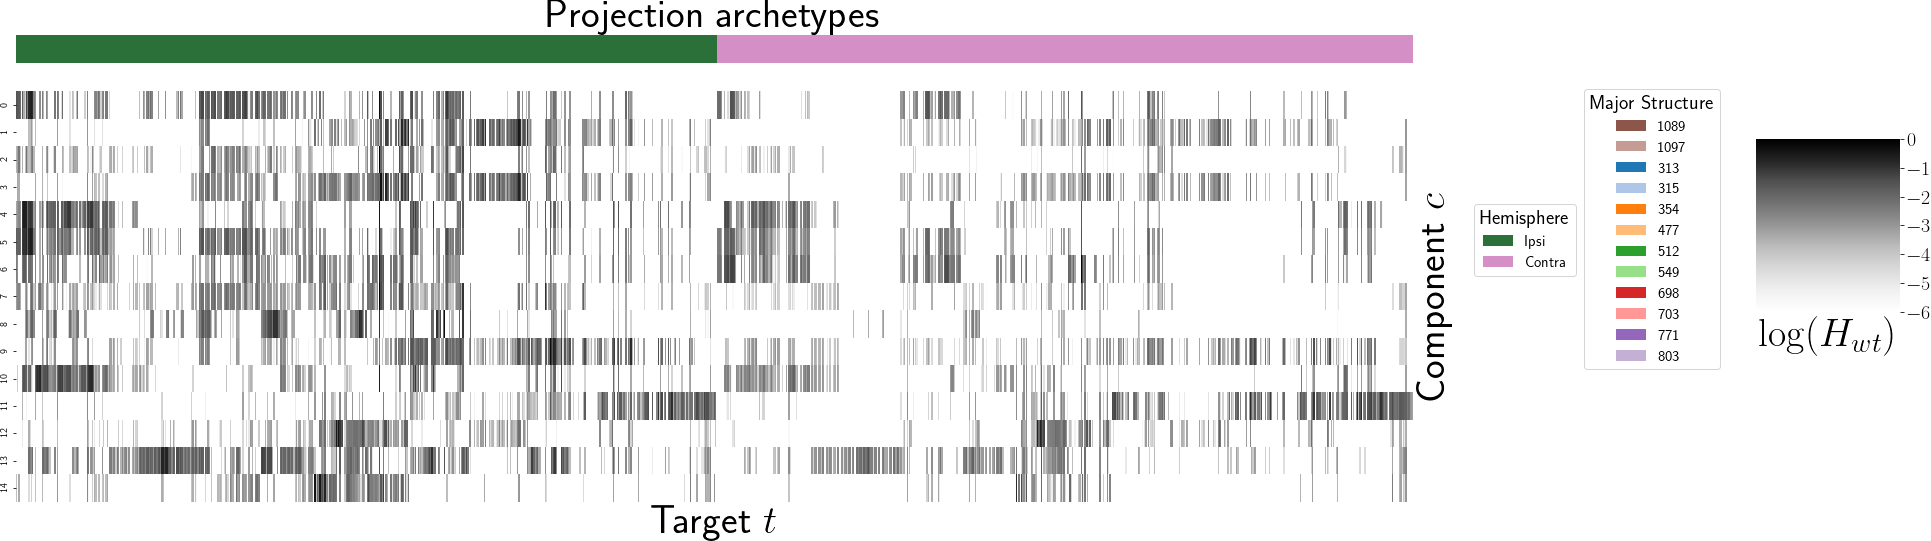
\includegraphics[width = .85 \textwidth]{figs/H_wt.png}
\label{fig:H}} 
\newline
\begin{tabular}[t]{cc}
\adjustbox{valign=t}{\subfloat[]{
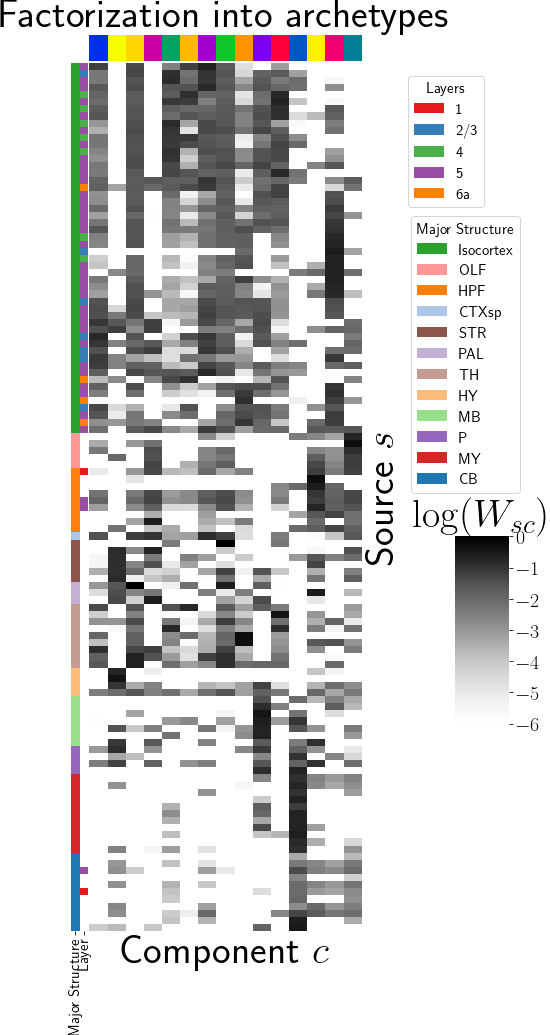
\includegraphics[width = .28\textwidth]{figs/W_wt.png}
\label{fig:W}}
} & 
\adjustbox{valign=t}{\subfloat[]{
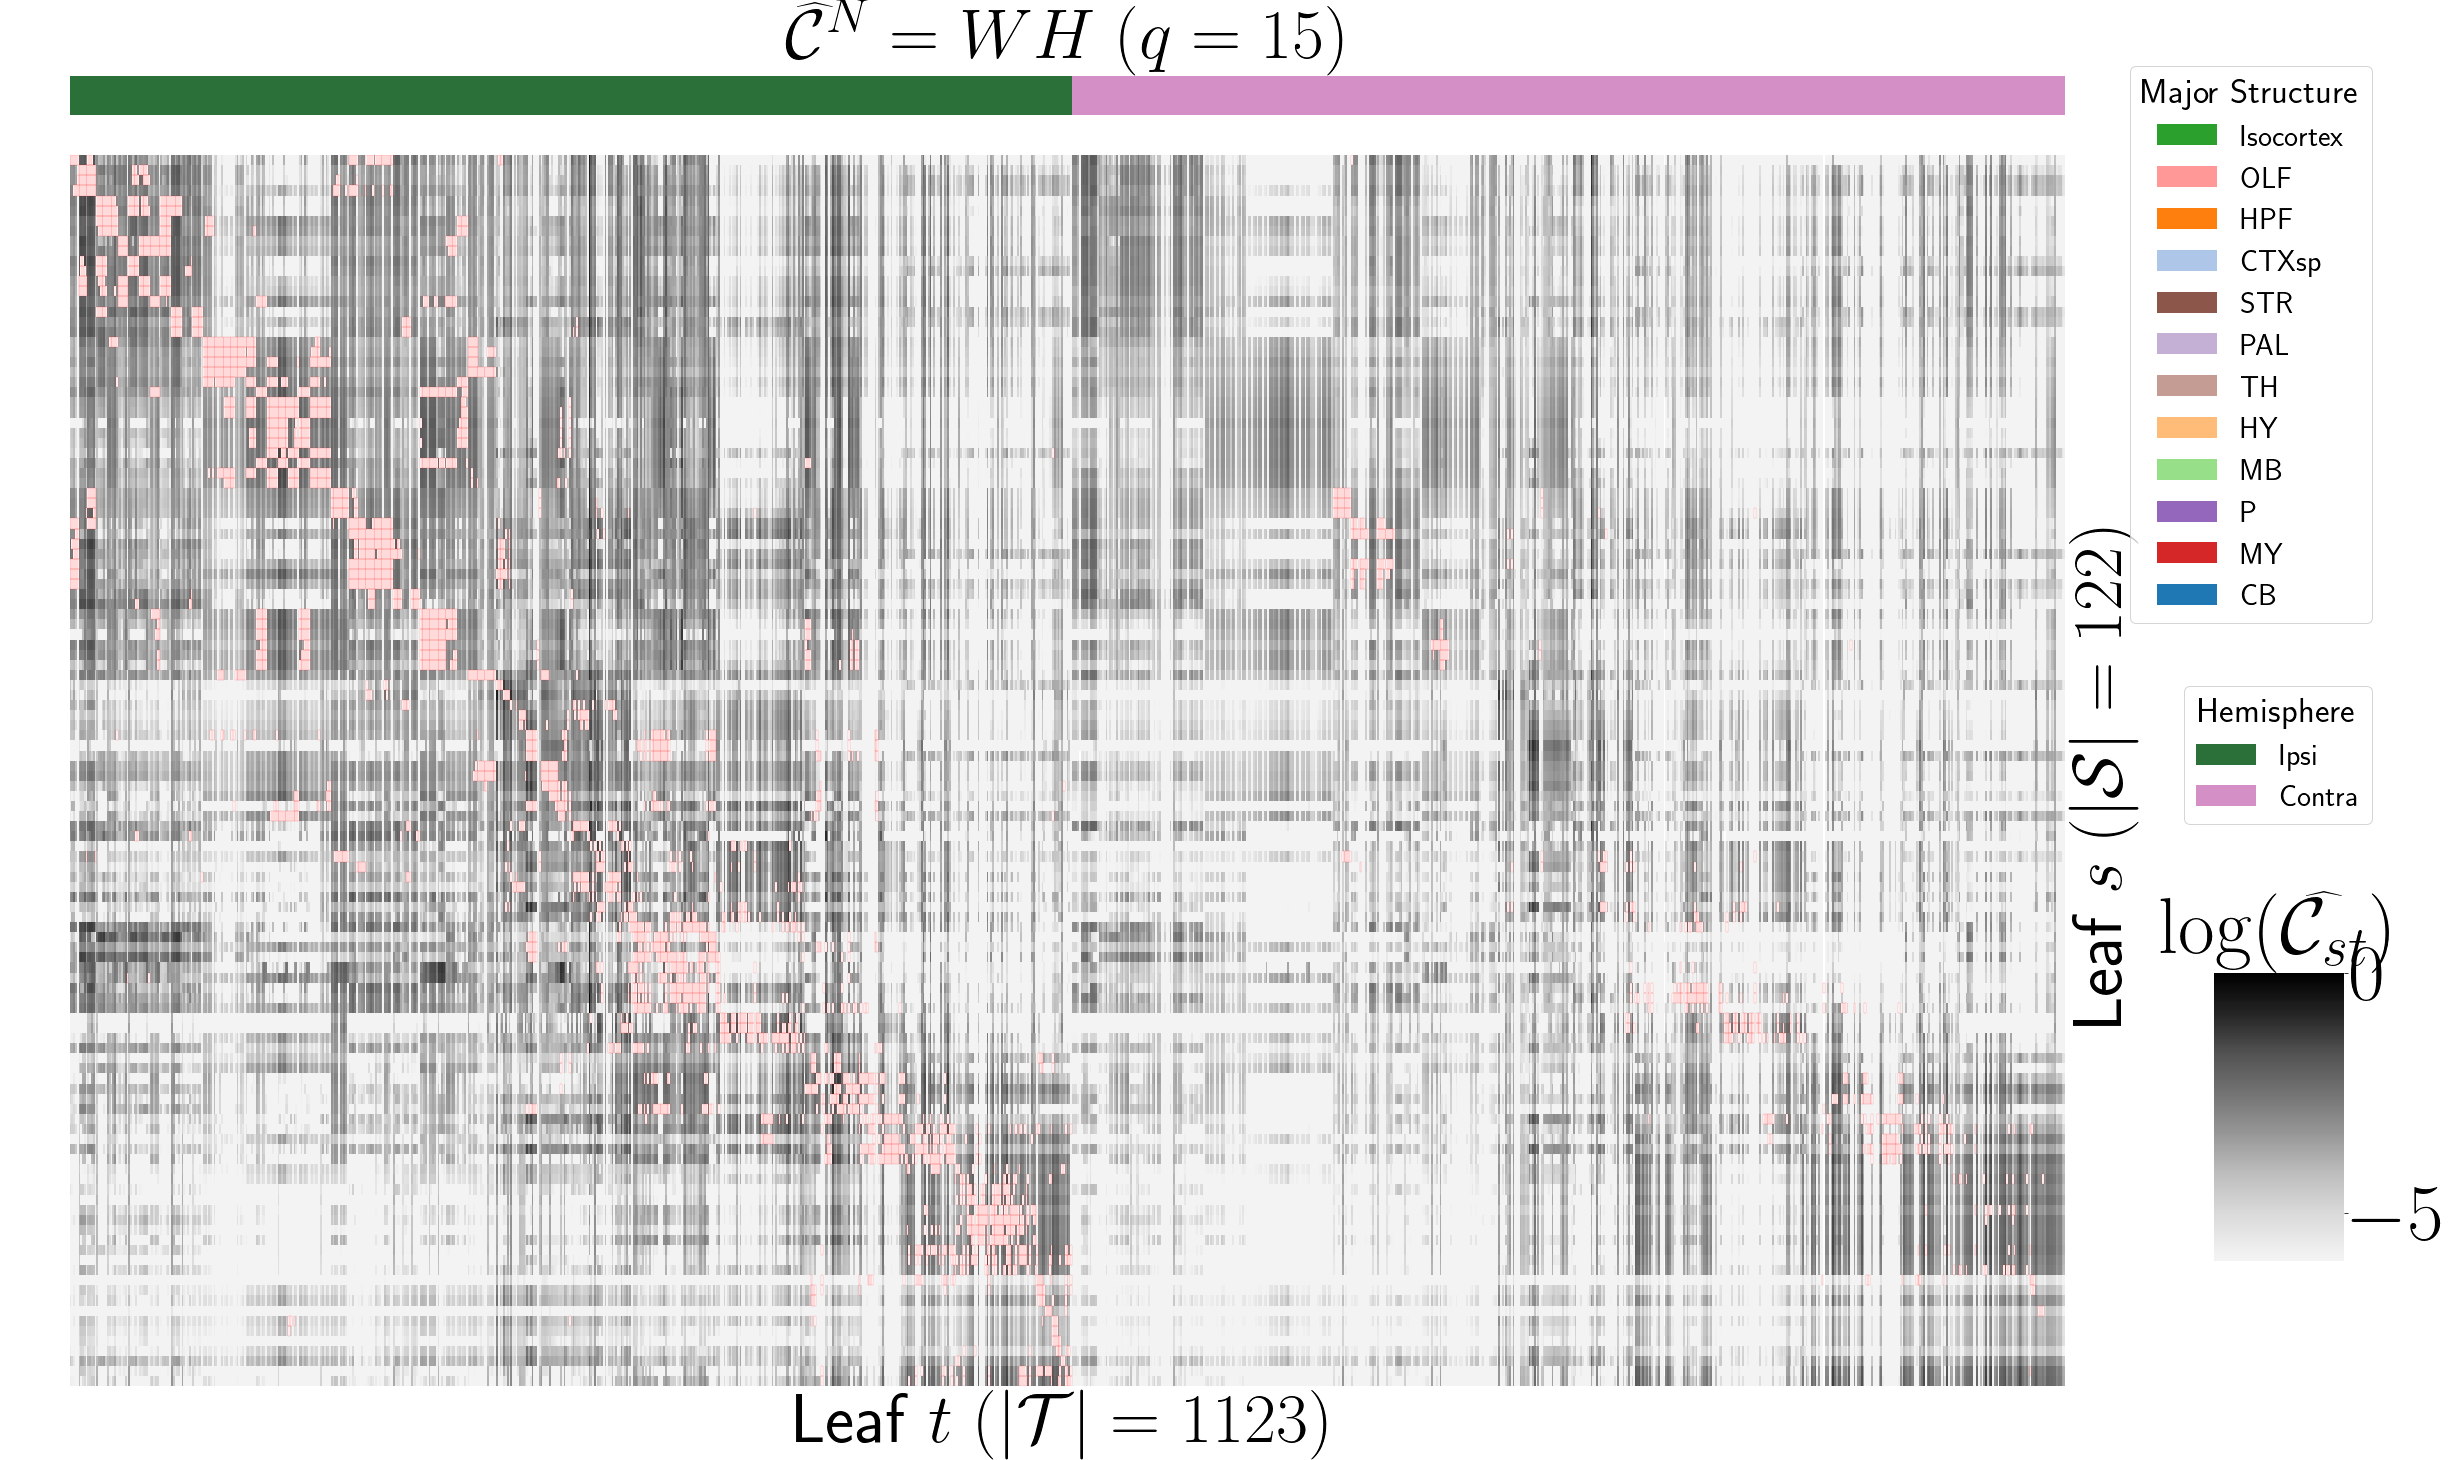
\includegraphics[width = .6\textwidth]{figs/conn_leafs_recon.png}
\label{fig:recon}}
} 
\end{tabular}
\caption{Non-negative matrix factorization results $\mathcal C_{wt}^N = WH$ for $q = 15$ components.
\ref{fig:H} Latent space coordinates $H$ of $\mathcal C$.
Target major structure and hemisphere are plotted.
\ref{fig:W} Loading matrix $W$.
Source major structure and layer are plotted.
\ref{fig:recon} Reconstruction of the normalized distal connectivity strength using the top $15$ archetypes.  Areas less than $1500 \mu m$ apart are not modeled, and therefore shown in red.
}
\label{fig:nmf_results}
\end{figure}

\newpage

